\documentclass[a4paper]{article}
\usepackage[utf8]{inputenc}
\usepackage[czech]{babel}
\usepackage[margin=13mm, tmargin=15mm, bmargin=12mm]{geometry}
\usepackage{multirow}
\usepackage{tikz}
\usetikzlibrary{calc}
\usepackage{chngpage}
\usepackage{tabularx}
\usepackage{fancyhdr}
\usepackage{mathptmx}
\usepackage{lipsum}
\usepackage{float}
\usepackage{longtable}

\renewcommand{\baselinestretch}{1.15}
\pagenumbering{gobble}
\pagestyle{fancy}
\renewcommand{\headrulewidth}{0pt}

\newcommand{\jmeno}{David Škrob, Tom\'{a}\v{s} N\'{a}zler, Vojtěch Nevrlý}
\newcommand{\trida}{L3A}
\newcommand{\poradovecislo}{}
\newcommand{\nazevulohy}{Pneumatika}
\newcommand{\cisloulohy}{}
\newcommand{\predmet}{Technické měření}
\newcommand{\skupina}{}
\newcommand{\datummereni}{8.6.2022}
\newcommand{\datumodevzdani}{14.6.2022}
\newcommand{\klasifikace}{}
\begin{document}
\fancyhead{
\begin{tikzpicture} [overlay,remember picture]
       \draw
        ($ (current page.north west) + (1cm, -12mm) $)
        rectangle
        ($ (current page.south east) + (-1cm,12mm) $);
\end{tikzpicture}
}

\renewcommand{\arraystretch}{2}
\shorthandoff{-}

{
\begin{adjustwidth}[]{-3mm}{-3mm}
\centering
\vspace*{-7mm}
\begin{tabularx}{\linewidth}{l|X|p{3cm}}
\multirow{2}{25mm}{\centering SPŠ a VOŠ technická Brno, Sokolská 1} &
\textbf{LABORATORNÍ CVIČENÍ Z ELEKTROTECHNIKY} & Třída: \trida \\
\cline{2-3}
 & Jméno a příjmení: \jmeno & Poř. Číslo: \poradovecislo \\
\hline
\end{tabularx}

\begin{tabularx}{\linewidth}{X|p{3cm}}
Název úlohy: \nazevulohy & Číslo úlohy: \cisloulohy \\
\hline
Zkoušený předmět: \predmet & Skupina: \skupina \\
\hline
\end{tabularx}

\begin{tabularx}{\linewidth}{X|X|X}
Datum měření: \datummereni &  Datum odevzdání: \datumodevzdani &  Klasifikace: \klasifikace \\
\hline
\end{tabularx}

\end{adjustwidth}
}

\shorthandon{-}

\section*{Zadání}
\newcounter{foo}
\setcounter{foo}{8}
 

\begin{itemize}
	\item [\arabic{foo}.] Vytvořte systém, který je schopen udržet jednu z dvou poloh po zmáčknutí tlačítka.
	\setcounter{foo}{9}
	\item [\arabic{foo}.] Vytvořte systém který bude posouvat pístem tam a zpět po zmáčknutí právě jednoho tlačítka.
\end{itemize}

\section*{Vypracování}



\begin{figure}[H]
	\centering
	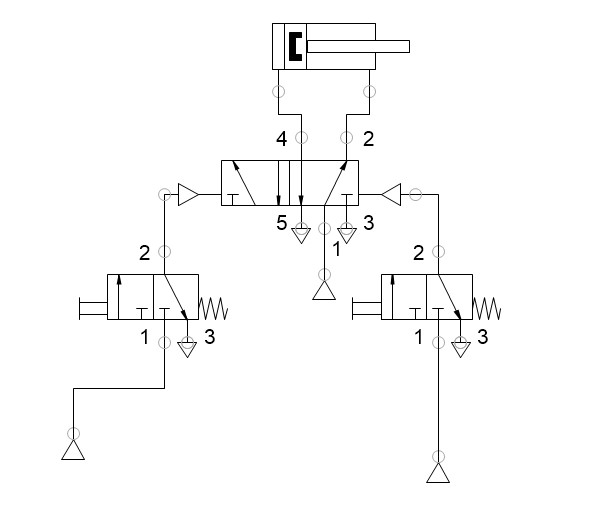
\includegraphics[width=0.75\textwidth]{lul.jpg}
	\caption{Řešení úlohy číslo 8.}
	\label{fig:mesh2}
\end{figure}

\begin{figure}[H]
	\centering
	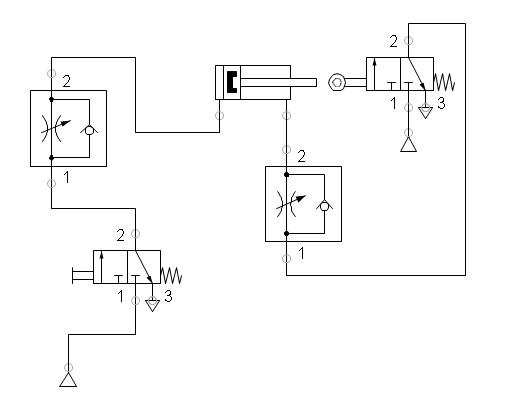
\includegraphics[width=0.75\textwidth]{lulwxd.jpg}
	\caption{Řešení úlohy číslo 9.}
	\label{fig:mesh1}
\end{figure}

\section*{Závěr}
Úloha číslo 8 byla velmi podobná jako úloha číslo 2, takže její řešení bylo jednoduché. Úloha číslo 9 byla již zajímavějši a složitější, ale i přes to jsme ji rychle vyřešili.
\section*{Použité pomucky:}
\begin{tabularx}{\linewidth}{c|c|c|l}
	Přístroj – pomůcka & Typ & Rozsah (pouze analogové)
	& Poznámka \\
	\hline
	Kompresor&&&\\
	\hline
	Dvoučinný píst& pneumatický&&\\
	\hline
	2 $\times$ Škrtící ventil&&&\\ \hline
	Rozvaděč&3/2&&Kontrolovaný mechanicky	\\ \hline
	2 $\times$ Rozvaděč&3/2&&Kontrolovaný tlačítkem	\\ \hline
\end{tabularx}
\end{document}